\section{Modus Operandi et implémentation}

Le développement a été réalisé sous vim en langage C, afin de profiter de la vitesse d'éxécution
ainsi que des optimisations de gcc à la compilation. D'un point de vue collaboratif, git a été
choisi pour sa facilité d'utilisation et l apossibilité d'héberger le code source et les documents
sur github.

Au niveau des choix d'implémentation, nous avons codé les graphes de manière à ce qu'il soit
possible d'utiliser une réprésentation en mémoire sous forme de matrice ou de liste
d'adjacence\footnote{Le choix de la représentation en mémoire est laissée à l'utilisateur et est
défini par les procédures utilisées pour la création des graphes.}. Chacun des algorithmes utilisés
requiérant un accès rapide aux voisins d'un noeud, nous avons choisi de représenter les graphes sous
forme de liste.

Nous avons créé un générateur de graphe aléatoire, garantissant la connexité du graphe généré. Le
générateur requiert pour s'éxécuter un nombre de n\oe uds et un nombre d'arêtes. A partir de ces
données, il crèe dans un premier temps un arbre contenant l'ensemble des n\oe uds du graphe puis par
une loi de probabilité défini le nombre de voisins de chacun des n\oe uds en s'assurant d'atteindre
exactement le nombre d'arêtes fixées.

Avec l'aide du générateur il est donc possible de générer des graphes de densité fixée. Cette
démarche permet l'expression du nombre d'arêtes en fonction du n\oe ud et vice versa et donc la
vérification des bornes calculées théoriquement précédemment.

Le programme de test génère un nombre donné de graphes aléatoires de densité fixée et applique
chacun des algorithmes sur ces graphes. Il calcule ensuite la moyenne des temps d'exécutions.

\section{Les résultats des tests}

\subsection{L'évolution du temps d'éxécution en fonction du nombre de n\oe uds}

Nous présenterons ici des résultats pour, respectivement, une densité faible, moyenne et grande.\\

\subsubsection{Densité $d = 2$ :}

\begin{figure}
\begin{center}
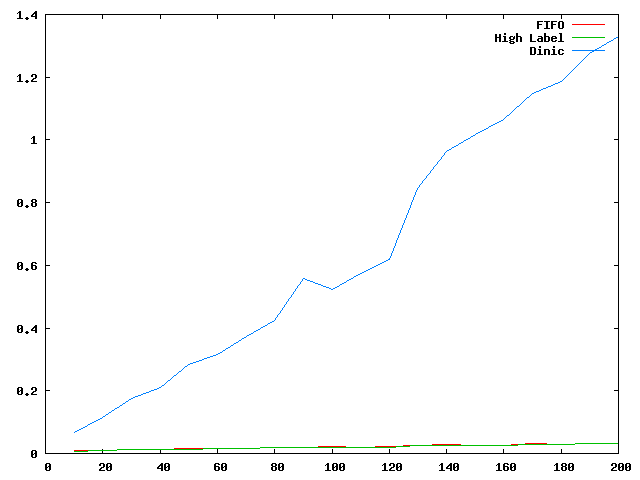
\includegraphics[scale=0.6]{../data_struct/results/ratio2.png}
\end{center}
\caption{Evolution du temps d'exécution des algorithmes en fonction du nombre de n\oe uds (densité =
2)}
\label{d2}
\end{figure}

Pour ce genre de densité, on a le nombre d'arêtes qui est du même ordre de grandeur que le nombre de
n\oe uds ce qui nous donne les complexités suivantes :
\begin{itemize}
\item Dinic $O(n^3)$
\item FIFO $O(n^3)$
\item High Label $O(n^2\sqrt{n})$
\end{itemize}

Malgré une complexité du même ordre de grandeur, l'agorithme FIFO s'exécute plus rapidement que
l'algorithme de Dinic, ce qui est du au fait que la borne supérieure de l'algorithme FIFO est très
rarement atteinte et que les cas où ce dernier est dit "lent" sont des cas pathologiques. On peut
remarquer aussi que l'algorithme High Label n'est un pas plus rapide que l'algorithme FIFO,
contrairement à ce que l'on pouvait escompter. Il est possible d'expliquer cette "mauvaise"
performance par un choix non adapté de structure de données.

En effet, lors du calcul de la complexité de ce dernier, nous avons estimé (implicitement) que le
temps d'accès au n\oe ud de plus grande distance n'influe pas sur la complexité de ce dernier. Or
ceci n'est vrai que si la structure de données utilisée pour stocker les sommets actifs est
correctement choisie. Lors de l'implémentation, nous nous sommes tourné ves un tas permettant un
accès en temps constant à la donnée recherchée. Seulement l'insertion et la suppression d'un n\oe ud
se font en $O(\log(n))$, ce qui augmente le temps d'exécution. Un choix judicieux aurait
été un tableau de listes chaînées~\cite{ahuj93} $t$ et l'utilisation d'une variable $k$ sauvegardant une borne
supérieure de la distance des n\oe uds. Ainsi, pour la sélection du n\oe ud de plus grand distance,
le tableau est parcouru en commençant par $t[k], t[k-1], \dots$, ce qui permet une insertion et une
suppression plus rapide.

\subsubsection{Densités $d=130$ et $d=200$}

\begin{figure}
\begin{center}
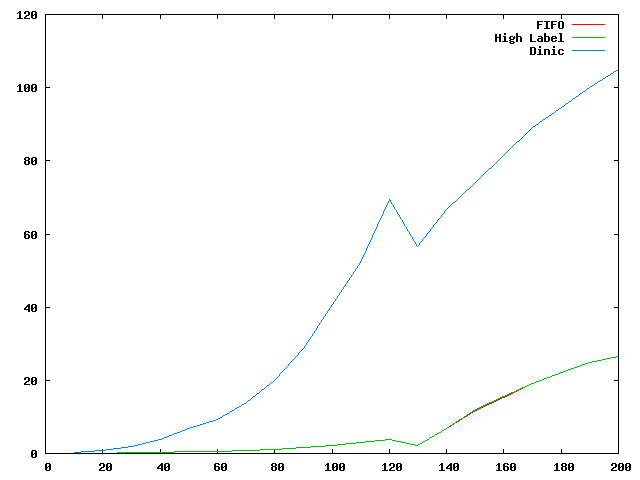
\includegraphics[scale=0.6]{../data_struct/results/ratio130.png}
\end{center}
\caption{Evolution du temps d'exécution des algorithmes en fonction du nombre de n\oe uds (densité =
130)}
\label{d130}
\end{figure}

\begin{figure}
\begin{center}
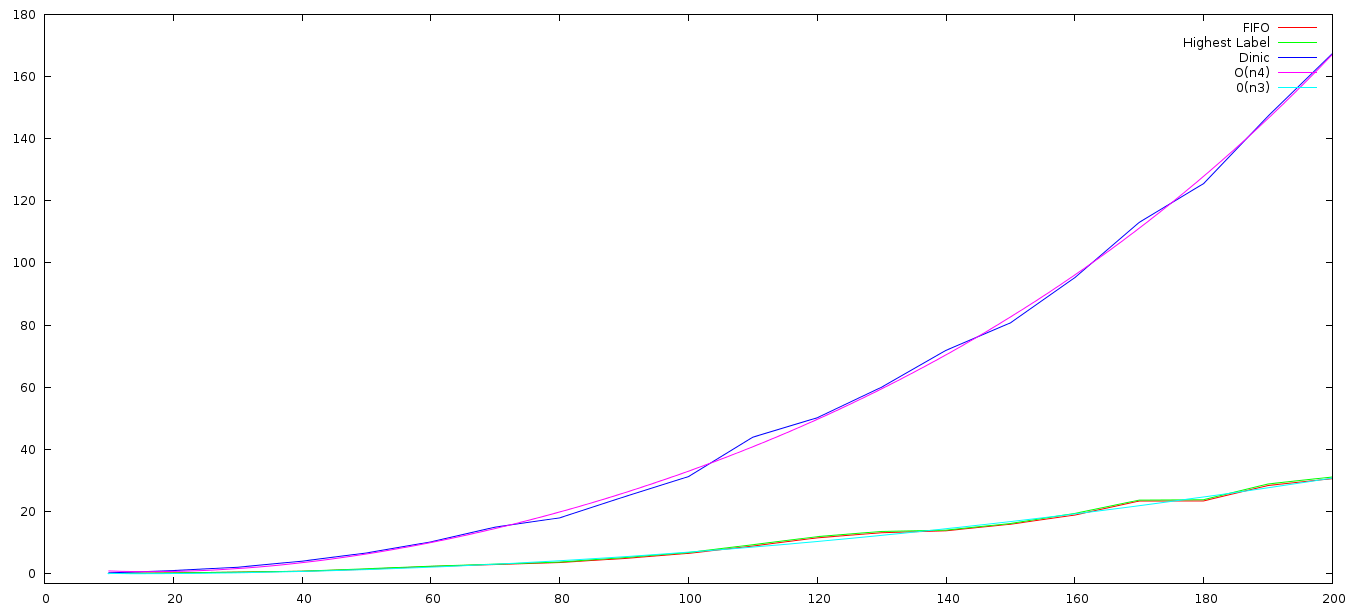
\includegraphics[scale=1.2]{../data_struct/results/ratio200b.png}
\end{center}
\caption{Evolution du temps d'exécution des algorithmes en fonction du nombre de n\oe uds (densité =
200)}
\label{d200}
\end{figure}

Lorsque la densité est grande, le nombre d'arêtes du graphe devient de l'ordre de $n^2$. On peut
alors espérer obtenir des complexités en $O(n^4)$ pour Dinic et $O(n^3)$ pour les algorithmes de
préflots.

Ce sont effectivement les résultats obtenus lorsque $d=200$, les courbes rajoutées correspondent aux
approximations données par gnuplot. Elles sont de la forme $P_1(x) = ax^4 + bx^3 +cx^2 +dx +e$ pour
Dinic et $P_2(x) = ax^3 + bx^2 + cx +d$ pour les algorithmes de préflots. Il est important de noter
que le coefficient $a$ est positif pour les deux plynômes ce qui prouve que la croissance de la
valeur du polynôme est de l'ordre du degré le plus élevé.

On observe, dans la majorité des cas, lorsque la densité est de l'ordre de $\frac{n}{2}$, une
brisure dans la courbe du temps des algorithmes. Nous n'avons aucune explication pour cette
dernière.

\subsection{Evolution du temps d'execution en fonction du nombre d'arêtes}


